\section{分类相关问题}
\subsection{多分类学习}
考虑用二分类学习器来解决多分类的问题。考虑$N$个类别$C_1,C_2,\cdots,C_N$,则将多分类任务拆分为若干个二分类任务求解,测试时,对这些分类器的预测结果进行集成,以获得最终多分类结果。
\subsubsection{一对一策略(One vs One,OvO)}
对给定数据集$D=\{(\sample{x}{1},\sample{y}{1}),(\sample{x}{2},\sample{y}{2}),\cdots,(\sample{x}{m},\sample{y}{m})\},\sample{y}{i}\in\{ C_1,C_2,\cdots,C_N \}$,OvO将$N$个类别两两配对,产生$\frac{N(N-1)}{2}$个二分类任务,其中,分类器把$D$中的$C_i$类样例作为正例,将$C_j$类样例作为反例。测试时,将新样本提交给所有分类器,得到$\frac{N(N-1)}{2}$个分类结果,最终结果通过投票产生。如下图所示
\begin{center}
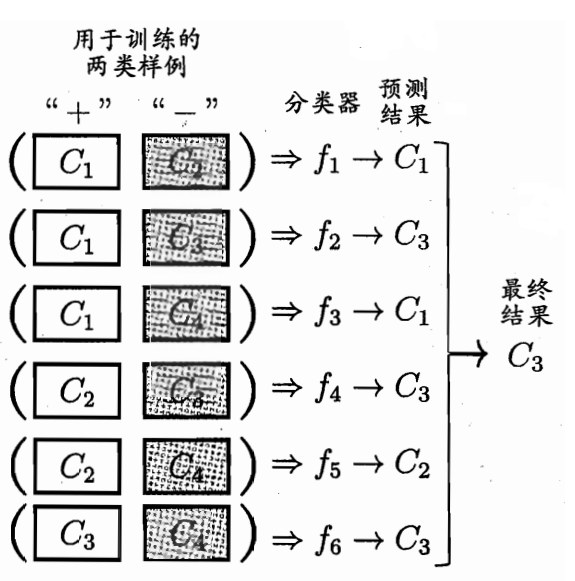
\includegraphics[scale=0.5]{../figures/CP1.PNG} 
\end{center}
可用矩阵来记录这个过程。初始化一个$N\times N$的0矩阵$A$。对于用来训练的两个样例$(C_i,C_j)$,若$C_i$为正例,$C_j$为反例,则记$A_{i,j}=1,A_{j,i}=0$;若$C_i$为反例,$C_j$为正例,则记$A_{i,j}=0,A_{j,i}=1$,如下
\begin{equation}
\begin{pmatrix}
0 & 1 & 0 & 1\\
0 & 0 & 0 & 1\\
1 & 1 & 0 & 1\\
0 & 0 & 0 & 0\\
\end{pmatrix}
\end{equation}
按行求和,可得到$(2,1,3,0)^T$,投票结果为$C_3$最多。则判断为$C_3$。
\subsubsection{一对其余策略(One vs Rest,OvR)}
OvR每次将一个类作为正例,其他类作为反例进行训练,得到$N个$分类器。测试时,若仅有一个分类器预测为正类,则对应的类别标记作为最终的分类结果;若有多个分类器预测为正类,则比较这些分类器的预测置信度,选择置信度最大的。

OvR只需要训练$N$个分类器,而OvO需要训练$\frac{N(N-1)}{2}$个分类器,因而OvO的存储开销和测试时间通常比OvR大,但由于OvO的每个分类器仅用到了两个类的样例,因而OvO的训练时间开销通常比OvR更小。

\subsection{类别不平衡问题}
对于二分类问题,若正例和反例的个数基本相等,对于一个线性分类器$y=f(x)$,则分类器决策规则为
\begin{eqnarray}
\begin{aligned}
\mbox{若}\frac{y}{1-y}>1 , \mbox{则预测为正例}
\end{aligned}
\end{eqnarray}
若正例和反例的个数不等,记$m^+$为正例数目,$m^-$为反例数目,则有
\begin{eqnarray}
\begin{aligned}
\mbox{若}\frac{y}{1-y}>\frac{m^+}{m^-} , \mbox{则预测为正例}
\end{aligned}
\end{eqnarray}
此时则需要对训练集进行调整。
\subsubsection{欠采样(undersampling)}
欠采样法若随机丢弃反例,则可能丢失一些重要的信息,常用的有EasyEnsemble算法。
\paragraph{EasyEnsemble算法}则是利用集成学习的机制,将多数类划分为若干个集合,使得这些多数类的子集中元素个数与少数类样本数量基本相同,供给不同学习器使用,最后将这些学习器集成起来。这样对每个学习器来看都进行了欠采样,但从全局来看,却不会丢失重要的信息。记多数类的样本集合为$L$,少数类样本集合为$S$,$N$为将多数类拆分成$N$个子集来训练$N$个分类器,算法如下
\begin{lstlisting}[language=python]
For i=1,`$\cdots$`,N
   (1) `随机从$L$中抽出样本构成多数类子集$L_1$,使得$|L_i|=|S|$`
   (2) `使用$L_i$和$S$的数据集,训练AdaBoost分类器$F_i$,其中$f_{ij}(x)$为弱分类器`
       `$$F_i(x)=sgn(\sum_{j=1}^n w_{ij}f_{ij}(x)-b_i)$$`
`将上述分类器联合起来`
`$$F(x)=sgn(\sum_{i=1}^N F_i(x))$$`
\end{lstlisting}

\paragraph{balance cascade}

\subsubsection{过采样(oversampling)}
若过采样法简单地对初始样本进行重复采样,很容易引起过拟合。一种方法是SMOTE算法,通过对训练集里的样本进行插值来产生额外的正例。
\paragraph{SMOTE算法}基本思想是根据少数类样本,生成新样本并添加到数据集中,步骤如下
\begin{itemize}
\item[1] 对于少数类$S$中每一个样本$x$,计算其到少数类样本集$S$中所有样本的距离,得到$K$个近邻;
\item[2] 根据样本不平衡比例里设置一个采样比例来确定采样倍率$N$,对于每一个少数类样本$x$,从其$k$近邻中随机选取若干个样本,假设选择的近邻为$\hat{x}$;
\item[3] 对于每一个随机选出的近邻$\hat{x}$,分别与原样本按照如下的公式构建新的样本
\begin{eqnarray}
x_{new}=x + rand(0,1)\times(\hat{x}-x)
\end{eqnarray}
其含义是在$x$和$\hat{x}$所成的线段上任取一个点。
\end{itemize}

该算法主要存在两方面的问题:一是在近邻选择时,存在一定的盲目性。从上面的算法流程可以看出,在算法执行过程中,需要确定$K$值,即选择多少个近邻样本,这需要用户自行解决。从$K$值的定义可以看出,$K$值的下限是$M$值($M$值为从$K$个近邻中随机挑选出的近邻样本的个数,且有$M < K$),$M$的大小可以根据负类样本数量、正类样本数量和数据集最后需要达到的平衡率决定。但K值的上限没有办法确定,只能根据具体的数据集去反复测试。因此如何确定$K$值,才能使算法达到最优这是未知的。 

另外,该算法无法克服非平衡数据集的数据分布问题,容易产生分布边缘化问题。由于负类样本的分布决定了其可选择的近邻,如果一个负类样本处在负类样本集的分布边缘,则由此负类样本和相邻样本产生的“人造”样本也会处在这个边缘,且会越来越边缘化,从而模糊了正类样本和负类样本的边界,而且使边界变得越来越模糊。这种边界模糊性,虽然使数据集的平衡性得到了改善,但加大了分类算法进行分类的难度.

\paragraph{Borderline-SMOTE1}记多数类的样本集合为$L$,少数类样本集合为$S$,$r=\frac{|S|}{|L|}$为少数类与多数类的比例。此算法用来提升SMOTE。步骤如下
\begin{itemize}
\item[1] 对于少数类$S$中每一个样本$x$,计算其到少数类样本集$S$中所有样本的距离,得到$K$个近邻,记该集合为$M_p$。计算样本$x$的这$K$个近邻属于$L$的数量,记为$m'=|M_p\cap L|$
\item[2] 若$m'=m$,则$x$是一个噪声点,不做任何操作;
\item[3] 若$0\leq m'\leq \frac{m}{2}$,说明$x$安全,不做任何操作;
\item[4] 若$\frac{m}{2}\leq m' \leq m$,则说明点$x$危险,需要在这个点附近生成一些新的少数类点,所以将它加入到集合$dange$中;
\item[5] 对于集合$danger$中的点$d$,使用SMOTE算法生成新的样本。
\end{itemize}

Borderline-SMOTE2与Borderline-SMOTE1很像,只是最后一步不一样。全部的步骤如下
\paragraph{Borderline-SMOTE2}记多数类的样本集合为$L$,少数类样本集合为$S$,$r=\frac{|S|}{|L|}$为少数类与多数类的比例。此算法用来提升SMOTE。步骤如下
\begin{itemize}
\item[1] 对于少数类$S$中每一个样本$x$,计算其到少数类样本集$S$中所有样本的距离,得到$K$个近邻,记该集合为$M_p$。计算样本$x$的这$K$个近邻属于$L$的数量,记为$m'=|M_p\cap L|$
\item[2] 若$m'=m$,则$x$是一个噪声点,不做任何操作;
\item[3] 若$0\leq m'\leq \frac{m}{2}$,说明$x$安全,不做任何操作;
\item[4] 若$\frac{m}{2}\leq m' \leq m$,则说明点$x$危险,需要在这个点附近生成一些新的少数类点,所以将它加入到集合$dange$中;
\item[5] 对于集合$danger$中的点$d$,分别在$S$和$L$中得到$k$个最近邻样本$S_k$和$L_k$。在$S_k$中选出$\alpha$比例的样本点和$d$作随机线性插值产生新的少数类样本。在$L_k$中选出$1-\alpha$比例的样本点和$d$做随机的线性插值产生新的少数类样本.
\end{itemize}
\subsubsection{权值移动(threshold-moving)}








